\documentclass{article}

\usepackage[margin=1in]{geometry}
\usepackage{amsthm}
\usepackage{amsmath,amssymb}
\usepackage{libertine}
\usepackage{bm}

\usepackage{fancyhdr}

\usepackage{graphicx}
\graphicspath{{./images/}}

\usepackage{longtable}
\usepackage{booktabs}
\usepackage{multirow}
\usepackage{subfig}
\usepackage{caption}
\usepackage{float}

\usepackage[hyphens]{url}
\usepackage{hyperref}
\hypersetup{breaklinks=true}

\usepackage{setspace}
\doublespacing

\usepackage{natbib}
\bibliographystyle{unsrtnat}
\setcitestyle{authoryear, open={(}, close={)}}

\begin{document}

\begin{titlepage}
    \begin{center}
        Modeling the Probability of a Successful Stolen Base Attempt in Major League Baseball \\
        \vspace{0.5cm}
        By \\
        \vspace{0.75cm}
        Cade Stanley \\
        \vspace{1.75cm}
        Submitted in Partial Fulfillment \\
        of the Requirements for \\
        Graduation with Honors from the \\
        South Carolina Honors College \\
        \vspace{1.5cm}
        May 2023 \\
        \vspace{1.5cm}
        Approved: \\
        \vspace{1.5cm}
        \rule{12cm}{0.4pt} \\
        Dr. Joshua Tebbs \\
        Director of Thesis \\
        \vspace{1.5cm}
        \rule{12cm}{0.4pt} \\
        Dr. Ting Fung Ma \\
        Second Reader \\
        \vspace{1.5cm}
        \rule{12cm}{0.4pt} \\
        Steve Lynn, Dean \\
        For South Carolina Honors College
    \end{center}
\end{titlepage}


\newpage
\begin{center}
    \section*{Abstract}
\end{center}
In Major League Baseball (MLB), the outcome of a stolen base attempt has important implications. Success moves the runner closer to scoring, while failure records an out and removes the runner from the basepaths altogether. Therefore, it is important that the decision by a coach or player to steal a base is well-informed. In this thesis, I explore a statistical approach to making this decision. I train logistic regression and random forest models, using data about the game situation and about the runner, pitcher, and catcher involved in the stolen base attempt, to estimate the probability that a stolen base attempt succeeds. With an estimated probability of success, MLB teams can make better decisions on the basepaths.
\addcontentsline{toc}{section}{Abstract}


\newpage
\tableofcontents


\newpage
\begin{center}
    \section{Introduction}
\end{center}
The basic goal in the sport of baseball is to score runs on offense and prevent runs on defense. Scoring runs can be accomplished singlehandedly (if a batter hits a home run), but it is more common for teams to score by putting runners on base and then advancing those runners. In most cases, a runner advances with the direct help of the batter at the plate – if the batter gets a hit, draws a walk, gets hit by a pitch, or puts a ball in play that leads to an error by the defense, the runner will likely advance. However, it is not uncommon to see a baserunner take matters into his own hands. A stolen base attempt is an effort by a baserunner to advance to the next base without the direct help of the batter. A runner may attempt to steal a base at any time, but in most cases, the runner attempts to steal as the pitcher is delivering a pitch. Once a pitcher starts his pitching motion, he is not allowed to stop it, meaning the runner can take off for the next base as soon as the pitcher begins his delivery. As a result, the runner has time to advance while the ball travels to home plate and while the catcher secures the ball and prepares to make a throw to stop the runner. 

In the larger context of a Major League Baseball (MLB) season, stolen base attempts may seem relatively unimportant. In fact, \cite{pavitt} shows that, among the categories of hitting, basestealing, pitching, and fielding, a team’s basestealing performance is easily the least important in explaining that team’s winning percentage over the course of a season. More specifically, and unsurprisingly, Pavitt concludes that hitting is much more informative than basestealing when using a team’s offensive performance to explain winning percentage. After all, stolen bases are far less common than hits, and stolen bases only allow a runner to advance one base. Hits are usually more productive, as they allow the batter to reach base and allow the runners already on base to advance, sometimes several bases at a time. \cite{baumer} also works to quantify the value of baserunning in baseball, finding that “the impact of baserunning upon a team’s run scoring ability is typically less than ±25 runs per season.” With a 162-game MLB season, this means that a team’s baserunning (not only its basestealing) accounts for less than one fifth of a run per game.

However, all of this is not to say that stolen base attempts are not worth studying. On a smaller scale, the outcome of a stolen base could certainly influence the events of the inning in which it occurs. A successful steal of second, for example, puts the runner in “scoring position,” where any hit is usually sufficient to score the runner. An unsuccessful steal, on the other hand, removes the baserunner from the basepaths and puts the batting team one out closer to the end of the inning. The characteristic of stolen base attempts which makes them most appealing as a subject of study, though, is the fact that every stolen base attempt is the result of a conscious decision made by a coach or player. As a result, it is worth investigating the kind of situations where a stolen base attempt is a good decision versus a bad one. It will be valuable to produce a quantitative tool for judging the feasibility of a stolen base attempt, as such a tool could be used to inform in-game decision making in baseball. 

Such uses of quantitative techniques to evaluate and assist with in-game decision making are widespread in the world of sports. For example, \cite{morris} provides a guide for the situations in which a two-point conversion attempt is warranted in the National Football League. \cite{bukiet} introduce a Markov chain model for the game of baseball and apply it to the selection of an optimal batting lineup. \cite{hirotsu} use a Markov decision process to estimate the value of a sacrifice bunt in the MLB, discussing whether it is worthwhile to sacrifice the batter for the purpose of advancing the baserunners. 

Regarding the subject of stolen bases, considerable work has been done to determine the minimum success rate needed for stolen base attempts to be worthwhile. It is generally accepted that stolen base attempts should be successful at least 75\% of the time for them to have a positive impact on a team’s offensive performance \citep{Stolen-Base-Percentage}.  This figure is derived using estimates of run expectancy from a given game situation (based on the number of runners on base and the number of outs) to measure the expected change in runs scored depending on the outcome of a stolen base attempt. \cite{keyes} provides an example of such a derivation and explains how the “breakeven” stolen base success rate changes with different game situations. With the knowledge that a success rate of about 75\% is needed for stolen base attempts to add value to the offense, the decision appears simple – send a runner to steal a base if he can do so successfully with a probability of at least 75\%. Of course, there will be more nuance to this decision depending on the game situation, and another question naturally arises – how can we predict the probability of success for any given stolen base attempt?

I propose multiple binary classification models, trained to classify stolen base attempts in Major League Baseball games as either successful or unsuccessful, using information about the runner, catcher, and pitcher involved in the stolen base attempt as well as the game situation at the time of the attempt. These models will be applicable to the prediction of stolen base outcomes on a case-by-case basis. With information about the probability of a stolen base attempt succeeding, as well as existing knowledge about the success rate needed for stolen base attempts to be worthwhile, a coach would have all the necessary information for deciding whether to send a runner. 

In building these models, it is reasonable to assume that the most important factors in the success of a stolen base attempt are the baserunner’s speed and the catcher’s arm strength. While this is likely true, there are several other factors that can influence the outcome of a stolen base attempt. For example, a baserunner will take a “lead” off of his base – before each pitch, he will take a few steps away from the base to give himself a head start for running. A larger lead creates a shorter distance between the runner and the next base, which improves the chance of a successful stolen base attempt. In addition, a runner’s timing and reaction time are extremely important. A runner is said to get a “good jump” on a stolen base attempt if he begins running right as the pitcher’s delivery begins. Even the smallest delay in the runner’s reaction could be the difference between reaching the next base safely and being thrown out. 

The pitcher also plays an important role in defending against stolen base attempts. In an attempt to shorten the runner’s lead, throw off the runner’s timing, or even get the runner out, a pitcher may make pickoff throws to the runner’s base, where a fielder will try to tag the runner out. If a pitcher is making frequent pickoff throws, the runner will have to stay closer to the base to avoid being thrown out, and the runner may have a harder time judging when the pitcher is beginning the motion of his delivery versus the motion of a pickoff throw. In general, left-handed pitchers have an advantage when defending against attempted steals of second base, as left-handed pitchers face first base when preparing to pitch. Left-handed pitchers can always keep an eye on the runner on first, while right-handed pitchers will have their backs turned to the runner. 

The pitch thrown as a runner is attempting to steal is very important as well. The faster a pitch reaches home plate, the sooner the catcher can make a throw to try to stop the runner. As a result, a stolen base attempt on a breaking ball or off-speed pitch may have a higher chance of success than a stolen base attempt on a fastball. The location of the pitch also matters. For example, a pitch in the dirt will be difficult for a catcher to corral, meaning it will take longer to try to throw out the runner. Occasionally, when a pitcher and catcher suspect that a runner will attempt to steal, the pitcher will throw a pitchout. This is a fast pitch purposefully thrown high and outside of the strike zone, allowing the catcher to catch the pitch standing up and to immediately make a throw to stop the runner. Throwing the ball outside of the strike zone is also meant to make the batter irrelevant in the play. When a pitch is inside of the strike zone, a batter may take a swing with the intention of distracting the catcher and disrupting the catcher’s timing.

Another important factor is the base that a runner is attempting to steal. Runners can attempt to steal second base, third base, or home plate, but steals of second are the most common. Since second base is the farthest base from home plate, stealing second gives a runner the most time to work with and puts the most pressure on the catcher to make a good throw. Attempted steals of home are quite rare, and their success typically relies on a lapse in focus by the pitcher or the catcher. Attempted steals of third base are more common than attempted steals of home, but they are considerably less common than steals of second, as stealing third base comes with a higher risk and a lower reward. Because the distance between home plate and third base is shorter than that between home plate and second base, it is easier for catchers to throw runners out at third. Furthermore, once a runner reaches second base, he is already in scoring position, so advancing from second base to third base does not generate as much value as does advancing from first to second. In short, attempted steals of second base are both the most common and the most interesting stolen base events, and so they will be the focus of this analysis.

All of these factors, including player attributes (a runner’s speed, a pitcher’s handedness, a catcher’s arm strength), the game situation at the time of a stolen base attempt, and the kind of pitch thrown as a stolen base attempt occurs, can be used to build classification models for the success and failure of stolen base attempts in Major League Baseball.



\newpage
\begin{center}
    \section{Methodology}
\end{center}

\subsection{Data Collection}
For this analysis, I gathered data from the 2018 MLB season, which is the most recent full season for which I was able to find easily accessible pitch data. With the need for information concerning the game situation, the players involved in the stolen base attempt, and the kind of pitches thrown, I gathered data from four different sources – Retrosheet’s play-by-play game files \citep{Retrosheet}, Paul Schale’s pitch data sets on Kaggle \citep{schale}, Baseball Savant’s Statcast data searching tools \citep{Statcast}, and Baseball Reference’s player data sets \citep{Baseball-Reference}. I wrote Python scripts in Jupyter Notebook (see Appendix A) to aid in the collection and cleaning of this data.

First, I used the Retrosheet game files to extract information about every attempted steal of second base during the 2018 MLB season. To begin, I wrote a Python script to identify every game and every inning in which a stolen base attempt occurred. The data was originally organized into team files for each of the thirty MLB teams, with each team file containing the data from each of that team’s home games. However, I only extracted the play-by-play data from the games containing a stolen base attempt, and I stored this data in individual files for each game. Unfortunately, the Retrosheet files only listed the plays that occurred over the course of each game, providing minimal information about the game situation for each play. The inning number (and whether it was the top or bottom half of the inning), the batter at the plate, and the number of balls and strikes were recorded for each play, but additional information such as the current pitcher, the current catcher, the names of any runners on base, and the number of outs, were not included. As a result, it was necessary to deduce this information for each stolen base attempt by recording every play leading up to the event and determining its effect on the game situation. Based on the formatting guidelines for the Retrosheet event files and the encodings used for every possible kind of play, I wrote a script that would update important aspects of the game situation according to the outcome of each play. Before every play, the script would record information such as the current pitcher and catcher (making note of any substitutions that occurred during the game), the number of runners on base and the names of those runners, the number of outs, and the number of balls and strikes in the at-bat. Other events leading up to the stolen base attempt, such as pitchouts or pickoff throws during the at-bat, were also noted. I ran this script on every game file containing a stolen base attempt, collecting plenty of information about the game status (and the plays leading up to that status) at the time of every attempted steal of second base during the 2018 MLB season.

With this information collected, I turned my attention to Schale’s Kaggle data set, which provided information about every pitch thrown during the 2018 season. This data did not include information about the outcome of each pitch, meaning there was no way to identify the pitches that occurred during a stolen base attempt by only observing the Kaggle data. However, the data did include information about the game and the at-bat during which each pitch occurred, and each pitch was labeled with its number in the at-bat. As a result, it was possible to merge the Kaggle pitch data with the Retrosheet stolen-base data according to the game situation at the time of the pitch and stolen base attempt. I wrote a Python script to merge these data sets on several variables, including the game in which the play/pitch occurred (based on the home team, the away team, and the date and start time of the game), the inning in which the play occurred, the number of outs when the play occurred, the pitcher and batter in the game when the play occurred, and the pitch number of the at-bat on which the play occurred. With this merge, I was able to match every stolen base attempt that occurred on a pitch with data about that pitch.  

The last type of data needed for building the model was the data on player attributes, such as a runner’s speed, a pitcher’s handedness, and a catcher’s arm strength. I used Baseball Savant’s Statcast search tool to download this data for every baserunner, pitcher, and catcher who participated in the 2018 season, and I merged this data with the Retrosheet stolen-base data based on the name and position of each player. For example, I merged the Statcast baserunner data with the Retrosheet stolen-base data based on the name of the runner who attempted each steal. Some player names were recorded differently between the two data sets, but the number of these discrepancies was small enough that it was possible to correct them by hand.  I also gathered Statcast data from the 2017 season, collecting information about each runner’s level of success in attempting steals and each pitcher’s success in preventing steals during that season. The Statcast data did not include similar information for catchers, but I was able to find this information on the Baseball Reference website. The purpose of gathering data from the 2017 season was to use players’ historical success with basestealing as a predictor in the model. Of course, not every player who was involved in a stolen base attempt during the 2018 season played during the 2017 season, so there was a considerable number of missing observations. I used mean imputation as a remedy for this.

Merging each of these different sources of data, I compiled a data set consisting of the following variables.
\begin{center}
    \begin{longtable}{c p{12cm}}
         \hline
         \textbf{Variable Name} & \textbf{Variable Description} \\ [0.5ex]
         \hline
         outcome & The outcome of the stolen base attempt -- success or failure. \\
         
         outs & The number of outs at the time of the stolen base attempt. \\
         
         b\_score\_difference & The difference between the score of the batter's team and the score of the pitcher's team at the time of the stolen base attempt. \\
         
         on\_third & An indicator of whether there was a runner on third base at the time of the stolen base attempt. \\
         
         num\_pitches & The number of pitches thrown in the at-bat before the stolen base attempt occurred. \\
         
         is\_hitters\_count & An indicator of whether the count of balls and strikes was favorable to the batter at the time of the stolen base attempt. \\
         
         is\_pitchers\_count & An indicator of whether the count was favorable to the pitcher at the time of the stolen base attempt. \\
         
         start\_speed & The starting speed of the pitch thrown as the stolen base attempt occurred. \\
         
         strike\_on\_event & An indicator of whether the pitch thrown during the stolen base attempt resulted in a strike. \\
         
         swing\_on\_event & An indicator of whether the batter swung at the pitch as the stolen base attempt occurred. \\
         
         pitchout\_on\_event & An indicator of whether the pitcher threw a pitchout as the stolen base attempt occurred. \\
         
         blocked\_on\_event & An indicator of whether the catcher had to block the pitch (i.e., if the pitch was thrown in the dirt) as the stolen base attempt occurred. \\
         
         pickoffs\_to\_first & The number of times that the pitcher attempted a pickoff throw to first base before the stolen base attempt occurred. \\
         
         pitchouts & The number of pitchouts that the pitcher threw during the at-bat before the stolen base attempt occurred. \\
         
         pitches\_run\_on & The number of pitches in the at-bat on which the baserunner attempted to steal. \\
         
         pitcher\_throws\_left & An indicator of whether the pitcher was left-handed. \\
         
         batter\_bats\_left & An indicator of whether the batter was left-handed. \\
       
         p\_sb\_rate\_2017 & The success rate of stolen base attempts against the pitcher during the 2017 season. \\
         
         p\_pickoff\_rate\_2018 & The success rate of the pitcher's pickoff throws during the 2018 season -- an indicator of the quality of the pitcher's pickoff move. \\
         
         r\_sb\_rate\_2017 & The baserunner's success rate on stolen base attempts during the 2017 season. \\
         
         r\_sprint\_speed\_2018 & The baserunner's average sprint speed during the 2018 season. \\
        
         c\_sb\_rate\_2017 & The success rate of stolen base attempts against the catcher during the 2017 season. \\
         
         c\_pop\_2b\_sba\_2018 & The catcher's average pop time on attempted steals of second base during the 2018 season. \\
         \hline

         \caption{Variable names and descriptions.}
         \label{tab1_variables}
    \end{longtable}
\end{center}

Each of these variables carries some potential significance in the outcome of a stolen base attempt. The number of outs at the time of a stolen base attempt, for example, may influence the aggressiveness of the pitcher and catcher in defending against the attempt. As an example, a runner on second base with no outs is more threatening than a runner on second base with two outs, so the defense may be more concerned about preventing a stolen base with no outs than they would be with two outs. Similarly, the score of the game could have some effect – pitchers and catchers are usually less concerned with preventing stolen base attempts in a blowout as compared to a competitive game. Whether or not there is a runner on third is very important – if the catcher attempts to throw out a runner who is stealing second, then a runner on third would have an opportunity to run for home plate. As a result, a catcher may not even attempt to prevent a runner from stealing second when there is a runner on third.

The number of pitches thrown during the at-bat has important implications for the runner’s timing. The more pitches a runner sees a pitcher throw, the better he can time the pitcher’s delivery to get a jump at the right moment. The count of balls and strikes would also be important because it may influence pitch selection. If the count is a “hitter’s count” (with more balls than strikes), the pitcher may be more likely to throw a fastball to make sure the pitch is in the strike zone. On the other hand, he may be more likely to deliver an off-speed pitch in a “pitcher’s count.” Given that the speed of a pitch partly determines how much time a runner has to steal second base, this influence of the count on a pitcher’s decision could be important. The result of the pitch thrown while the runner is attempting to steal is also significant. As mentioned above, a faster pitch gives the runner less time to reach second base. A pitch in the strike zone may be easier for the catcher to handle and quickly throw to second compared to a pitch outside of the strike zone. If the catcher has to block the pitch, it will likely be difficult to throw the baserunner out. And, as previously discussed, the batter swinging at the pitch could disrupt the catcher’s timing and make it easier for a runner to steal, while the pitcher throwing a pitchout would likely make it easier for the catcher to throw the runner out.

Other events occurring throughout the at-bat may also influence the prospects of a successful stolen base attempt. If the pitcher makes several pickoff throws, the runner may be forced to stay closer to first base and may be unable to get a good jump on a stolen base attempt. If the pitcher throws pitchouts during the at-bat, this may be an indication that he is very aware of the baserunner and very concerned with preventing a stolen base by any means necessary. The number of pitches in the at-bat on which the runner attempts to steal may also be useful, as more attempts at stealing could allow the baserunner to better time the pitcher’s delivery and to get a better jump.

The handedness of the pitcher and the batter are additional important factors. The pitcher’s handedness is especially meaningful because a left-handed pitcher stands facing the runner on first base, whereas a right-handed pitcher has his back to the runner. The handedness of the batter may influence the catcher’s attempted throw to second base. Every catcher who played in the 2018 MLB season was right-handed, so batters standing in the right batter’s box (that is, left-handed batters) may sometimes be in the way of a catcher attempting to throw a runner out at second base.

The final variables considered are those that measure several player attributes that directly relate to stolen base attempts. Stolen base success rates from the 2017 season may indicate how well a runner steals bases or how well a pitcher or catcher defends against stolen base attempts. A runner’s sprint speed will certainly influence the success of a stolen base attempt, as will a catcher’s average pop time (the time it takes between the catcher receiving the pitch and the ball reaching second base). The success rate of a pitcher’s pickoff throws during the 2018 season is meant to capture the quality of the pitcher’s “pickoff move.” Runners may be more cautious against a pitcher with a good pickoff move, which could make a successful stolen base attempt less likely.

Some of these variables appear only tangentially related to the outcome of a stolen base attempt, while others have a much clearer role. However, it is worth considering all of these variables in an effort to maximize the predictive ability of the classification models. Variable selection will be used to trim useless predictors.


\subsection{Data Analysis}
With the data collected and cleaned, I used two approaches to building a model – logistic regression and random forests (see Appendix C and Appendix D for a discussion of these two classification methods). For each approach, I also utilized two different data sets. The first was the full data set, including every variable described in the above table. In this data set, the variables documenting the outcome of pitches thrown during a stolen base attempt offer both advantages and disadvantages. The primary advantage is that they represent predictors that can be directly connected to the outcome of a stolen base attempt. The speed of the pitch, whether the pitch was a pitchout, or whether the pitch needed to be blocked by the catcher, for example, all possess clear connections to the success or failure of a stolen base attempt. As a result, including these variables in the models could potentially improve prediction accuracy.

However, these variables also come with two notable drawbacks. The first is that they give rise to missing values in the data set. Although most stolen base attempts occur during the delivery of a pitch, there were 201 attempts during the 2018 season (out of 2867 total attempted steals of second base) which did not occur on a pitch, usually because the pitcher caught the runner with a pickoff move. As a result, the full data set contains 201 missing observations which need to be removed. The second drawback of the pitch variables is that they contain information that is unavailable for live, in-game decision making. Although the pitch variables make sense as predictors, a coach or player deciding to attempt a stolen base would not know anything about a pitch which has not happened yet. They could speculate, using factors such as the count of balls and strikes to guess the kind of pitch about to be thrown (fastball or off-speed), and they could decide beforehand whether the batter will swing at the pitch, but these methods would be inexact. If these models are to be used as decision-making tools, it is important that they are trained only on data that would be available at the time a decision is made. Therefore, for the second data set, I excluded the five variables that document the outcome of a pitch – “start\_speed,” “strike\_on\_event,” “swing\_on\_event,” “pitchout\_on\_event,” and “blocked\_on\_event.” Unfortunately, the method I used to record the score of the game at the time of a stolen base attempt also depended on the Kaggle pitch data, so the “b\_score\_difference” variable also had to be dropped for this second data set.

For each of the two data sets, I fit a logistic regression model and a random forest classifier. For each logistic regression model, I began by including all of the variables from the given data set as predictors, in addition to three interaction terms – one between the pitcher's stolen-base success rate and the runner's stolen-base success rate, one between the catcher's stolen-base success rate and the runner's stolen-base success rate, and one between the catcher's pop time and the runner's sprint speed. I then applied a stepwise approach to variable selection, using the Akaike information criterion (AIC) to identify the subset of predictor variables that produced the highest quality model in terms of prediction error. For each random forest, I included all of the variables from the given data set (either the full data set or the data set excluding pitch information). 

After fitting the best two logistic regression models and training the two random forests, I evaluated their predictive performance using cross-validation techniques. For the logistic regression models, leave-one-out cross-validation was feasible, but this technique was too computationally expensive when applied to the random forests. As a result, I used five-fold cross-validation for the random forests. Using the cross-validated prediction results, I produced a Receiver Operating Characteristic (ROC) curve and a confusion matrix, and I calculated the area under the curve (AUC) and the prediction accuracy, for each of the four models. These results are summarized in the next section. 



\newpage
\begin{center}
    \section{Results}
\end{center}
%\begin{center}
    \begin{longtable}{c c c|c c}
        \toprule
        & \multicolumn{2}{c}{Including Pitch Data} & \multicolumn{2}{c}{Excluding Pitch Data} \\
        \cmidrule{2-3} \cmidrule{4-5}
        & Logistic Regression & Random Forest & Logistic Regression & Random Forest \\
        AUC & \textbf{0.6915} & 0.6561 & 0.6759 & 0.6638 \\
        Prediction Accuracy & 0.7611 & \textbf{0.7613} & 0.7245 & 0.7361 \\
        Sensitivity & 0.9678 & \textbf{0.9684} & 0.9585 & 0.9400 \\
        Specificity & 0.1574 & 0.1564 & 0.1381 & \textbf{0.2253} \\
        \bottomrule
        \caption{Measures of model performance, compared across data sets and model types.}
        \label{tab2_results}
    \end{longtable}
%\end{center}

When making predictions using each model, I used a cutoff value of 0.5. That is, if the expected probability of success produced by the model was at least 0.5, then the stolen base attempt was predicted to be successful. With this approach, I generated a confusion matrix for each model (see Figure \ref{fig3_conf} and Figure \ref{fig4_conf} in Appendix B), from which I calculated the model's accuracy, sensitivity, and specificity. Accuracy is the overall proportion of stolen base outcomes that the model correctly classifies, sensitivity is the proportion of successful stolen base attempts that the model correctly classifies as successful, and specificity is the proportion of unsuccessful stolen base attempts that the model correctly classifies as unsuccessful. Each model performs well in terms of overall classification accuracy, with over 70\% of stolen base outcomes predicted correctly. The models are very good at correctly classifying successful stolen base attempts (as evidenced by the high sensitivity values), but they are quite poor at correctly classifying unsuccessful stolen base attempts (as evidenced by the low specificity values). This is important to note, as an unsuccessful stolen base attempt generally does more harm to an offense than a successful stolen base attempt does good. This is because a successful stolen base attempt simply advances a runner by one base, while an unsuccessful attempt both removes the runner from the basepaths and adds an out. For example, using Greg Stoll’s expected runs calculator \citep{stoll}, we can consider the situation of a runner on first with no outs. A successful stolen base attempt by this runner adds approximately 0.25 expected runs for the offense, whereas an unsuccessful attempt subtracts about 0.61 expected runs. Therefore, misclassifying an unsuccessful stolen base attempt as successful is a more costly error than misclassifying a successful attempt as unsuccessful. As a result, it would be worthwhile to aim for a higher specificity from these models, which could be achieved by increasing the cutoff value required to classify a stolen base attempt as successful. Finding an optimal cutoff value for each model would be a valuable subject of future study.

Compared to the accuracy, specificity, and sensitivity metrics, a more comprehensive measure of each model’s quality is its AUC score, which is calculated from the model's ROC curve (see Figure \ref{fig1_roc} and Figure \ref{fig2_roc} in Appendix B). Using this score, the best overall model is the logistic regression model trained on the full data set (including the pitch data). Across both the full data set and the reduced data set, logistic regression performs better than a random forest. And, somewhat surprisingly, both the logistic regression model and the random forest built without the pitch data perform better than the random forest built using the full data set. With each model exhibiting an AUC score between 0.65 and 0.70, we can say that these models perform somewhat well. At the very least, they perform better than an approach that classifies stolen base outcomes at random (which corresponds to an AUC score of 0.5), but their performance is not exceptional by any means. Again, each model performs well at correctly classifying successful stolen base attempts, but there is room for improvement in the classification of unsuccessful attempts.

Not only are these models interesting for their predictive capabilities, but they can also provide information on the importance of each variable in explaining the outcome of a stolen base attempt. For the logistic regression models, the primary indication of whether a variable is important is whether it is included in the model with the lowest AIC score (using the stepwise approach). The variables included in the best model for the full data (with pitch data) and the variables included in the best model for the reduced data (without pitch data) can be seen in Table \ref{tab3_logistic_summary} and Table \ref{tab4_logistic_summary}, respectively, of Appendix B. These tables also include the p-value for each variable, which acts as another indicator of the variable's importance -- a lower p-value indicates a larger significance in the model. For the logistic regression models, some of the most significant factors in explaining the outcome of a stolen base attempt are the number of pitches thrown during the at-bat, the speed of the pitch thrown during the stolen base attempt, the baserunner's average sprint speed, whether a runner is on third at the time of the attempt, whether the count is favorable to the batter at the time of the attempt, and whether the catcher has to block the pitch during the stolen base attempt. For each of these variables, we can also examine the estimate of its coefficient in the logistic regression model to understand how it is related to the probability of a successful stolen base. The presence of a runner on third, for example, corresponds with a higher probability that a stolen base attempt is successful, holding constant every other variable in the model. A count of balls and strikes that is favorable to the batter is also positively associated with success, as is the baserunner's sprint speed. On the other hand, the speed of the pitch thrown during the stolen base attempt is negatively related to the probability of success -- the faster the pitch, the less likely the stolen base attempt will be successful.

The random forests also possess indicators of the importance of each variable, seen in Table \ref{tab5_importance} and Table \ref{tab6_importance} of Appendix B. Each table contains two metrics that measure variable importance, with higher scores for these metrics indicating that a variable is more important for classifying stolen base outcomes in the random forest model. Across the two random forests, some of the most important factors include the number of pitches in the at-bat leading up to the stolen base attempt, the speed of the pitch thrown during the stolen base attempt, and whether there is a runner on third at the time of the attempt. These factors were similarly important in the logistic regression models. Other variables of notable importance in the random forests are the variables documenting characteristics of the pitcher, baserunner, and catcher involved in the stolen base attempt. Each player's success rate from the 2017 season carries considerable importance in the models, as does the pitcher's rates of fastballs and successful pickoff throws, the baserunner's average sprint speed, and the catcher's average pop time. The importance of these kinds of variables is notable because it indicates that player attributes and historical stolen base data are quite useful in explaining the outcomes of future stolen base attempts.

So, not only can these logistic regression models and random forests serve as practical decision tools that perform better than random decision-making, but they also provide insight into the factors that are most important to consider when weighing the viability of a stolen base attempt.


\newpage
\begin{center}
    \section{Conclusion}
\end{center}
Ultimately, these classification models (in particular, the models excluding the pitch data) could act as in-game decision-making tools that, while not perfectly reliable, are better than deciding to attempt a stolen base at random. In fact, the primary value of these models may come not from their binary classification results, but from their estimated classification probabilities. Using a tool like Greg Stoll’s expected runs calculator, the estimated probability of success for a stolen base attempt could be used to estimate the expected change in a team’s expected runs resulting from a stolen base attempt. Returning to the previous example of a runner on first and no outs, a successful stolen base attempt would add about 0.25 expected runs, while an unsuccessful attempt would subtract about 0.61 expected runs. In this case, a stolen base attempt would need a probability of success of at least $\frac{61}{86} \approx 0.71$ in order for the expected change in expected runs to be nonnegative. A simple decision rule, then, would be to send the runner if the estimated probability of success produced by the model is at least 0.71.

Future research in this area should focus primarily on improving model performance. One potential avenue for this is in the use of other kinds of classification models, such as support vector machines, k-nearest neighbors classifiers, or neural network classifiers. It would also be worth re-examining the predictors included in the model and searching for other valuable predictors that may be added. For example, instead of calculating players’ historical rates of stolen-base success using only the 2017 season, it may be more useful to use a player’s entire career. This would reduce the number of missing values in the data set (from players who did not play during the 2017 season) and would provide a larger sample of data for evaluating a player’s ability to successfully steal bases (or defend against stolen base attempts). 

In terms of new predictors to add, both the length of a pitcher's delivery and the length of a runner's lead could be valuable additions. The length of a pitcher’s delivery is the amount of time it takes for the pitcher to release the ball after beginning his pitching motion, so this variable directly influences the amount of time a runner has to steal. This kind of information may already be captured by measuring the historical success rate of stolen base attempts against a given pitcher, and this kind of data would be difficult to collect, but it may be worth investigating. The length of a runner's lead off of his base may also influence the likelihood of a successful stolen base attempt, as the lead distance directly determines the distance the runner has to cover when attempting to steal. A larger lead creates a shorter distance to the next base, but it also increases the risk that the runner is picked off by the pitcher. Similar to data about the length of a pitcher's delivery, data about the length of a runner's lead would be difficult to measure and collect. Furthermore, when using these models for decision making, it would be impossible to measure a runner's lead distance in real time to include it in the models. A runner's lead is constantly changing, and it is likely based more on feel than on a careful consideration of the exact distance covered. Regardless of their potential drawbacks, these two variables are examples of factors not explored in this project that would be interesting subjects of future study.

Another important consideration for future research involves several rule changes that took effect at the beginning of the 2023 MLB season. Most notably, when there is a runner on base, pitchers are allowed to perform a maximum of two pickoff attempts per plate appearance. Furthermore, the sizes of first, second, and third base were increased from fifteen inches on each side to eighteen inches on each side. Both of these rule changes will be advantageous to baserunners attempting to steal. The limit on pickoff throws will allow runners to be more aggressive when taking a lead, especially if the pitcher has already attempted two pickoff throws. While a third pickoff throw is technically allowed, it must occur on a play where either the runner advances a base or is thrown out. If the pitcher's third pickoff attempt is unsuccessful, the runner is given a free advance to the next base. The increase in the size of each base also provides a small advantage to baserunners, as it slightly reduces the distance the runner needs to cover during a stolen base attempt. Additionally, sliding into a base (and staying on the base through the slide) will be easier with larger bases. With these rule changes, it will be worthwhile to revisit this analysis in the future and determine whether the probability of success for stolen base attempts has increased across the board.

Overall, the logistic regression models and random forests presented here establish a good baseline for the classification of stolen base outcomes in Major League Baseball. They represent a good first step in the construction of decision tools that can be used by coaches and players in a live game, but there is ample room for future research and improvement.



\newpage
\bibliography{references}
\addcontentsline{toc}{section}{References}



\newpage
\begin{center}
    \section*{Appendix}
\end{center}
\addcontentsline{toc}{section}{Appendix}
\appendix

\subsection*{Appendix A: Code and Data}
The data sets, Python scripts, and R code used to produce this thesis can be found at \url{https://github.com/cadets1/senior\_thesis}.
\addcontentsline{toc}{subsection}{Appendix A: Code and Data}


\subsection*{Appendix B: Figures and Tables}
\addcontentsline{toc}{subsection}{Appendix B: Figures and Tables}
\begin{figure}[h]
    \centering
    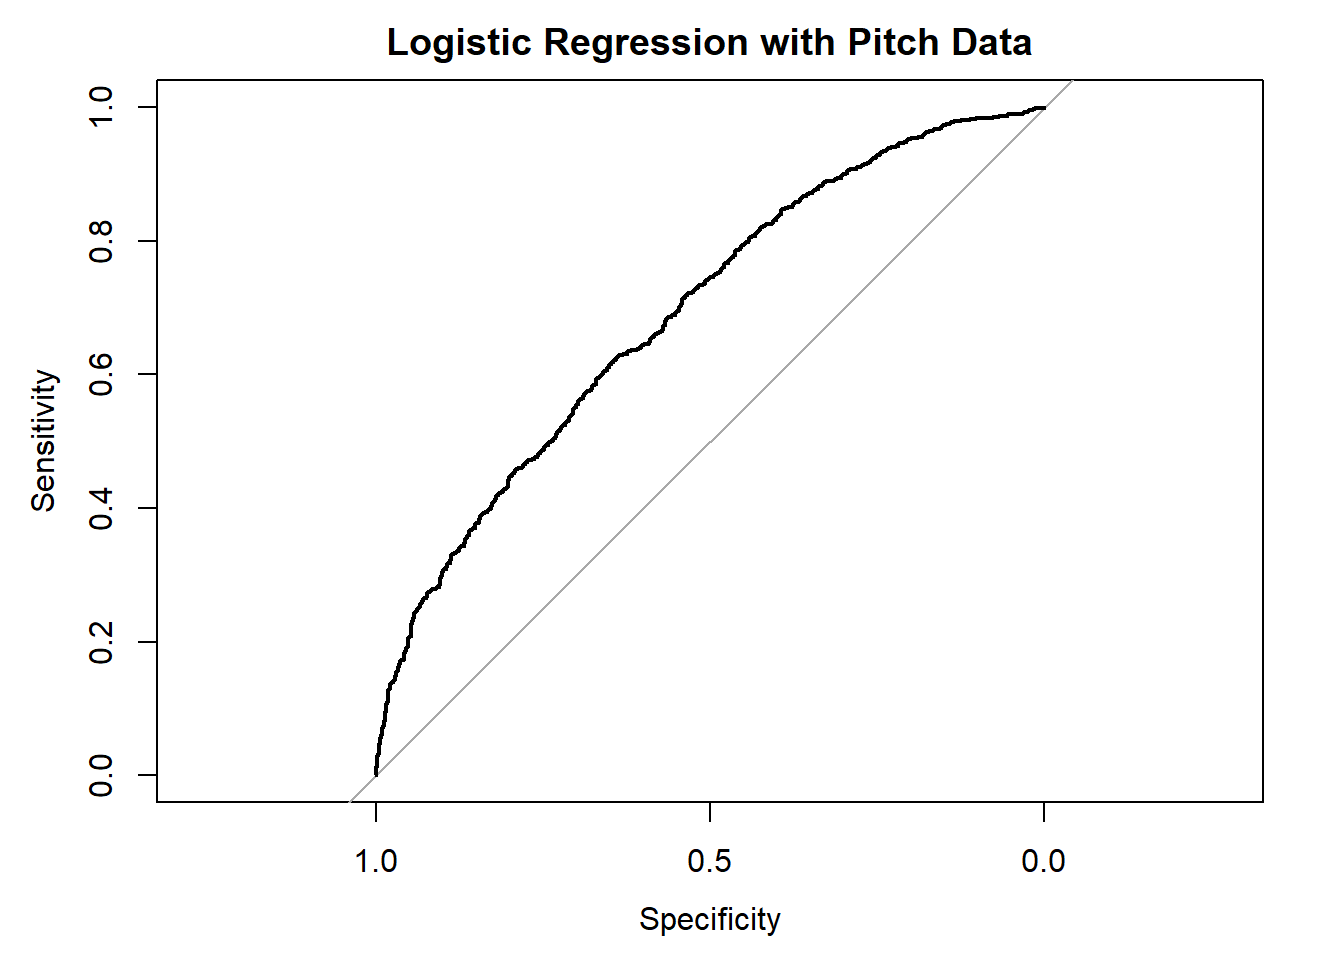
\includegraphics[height=2in]{images/reduced_glm_roc.png}
    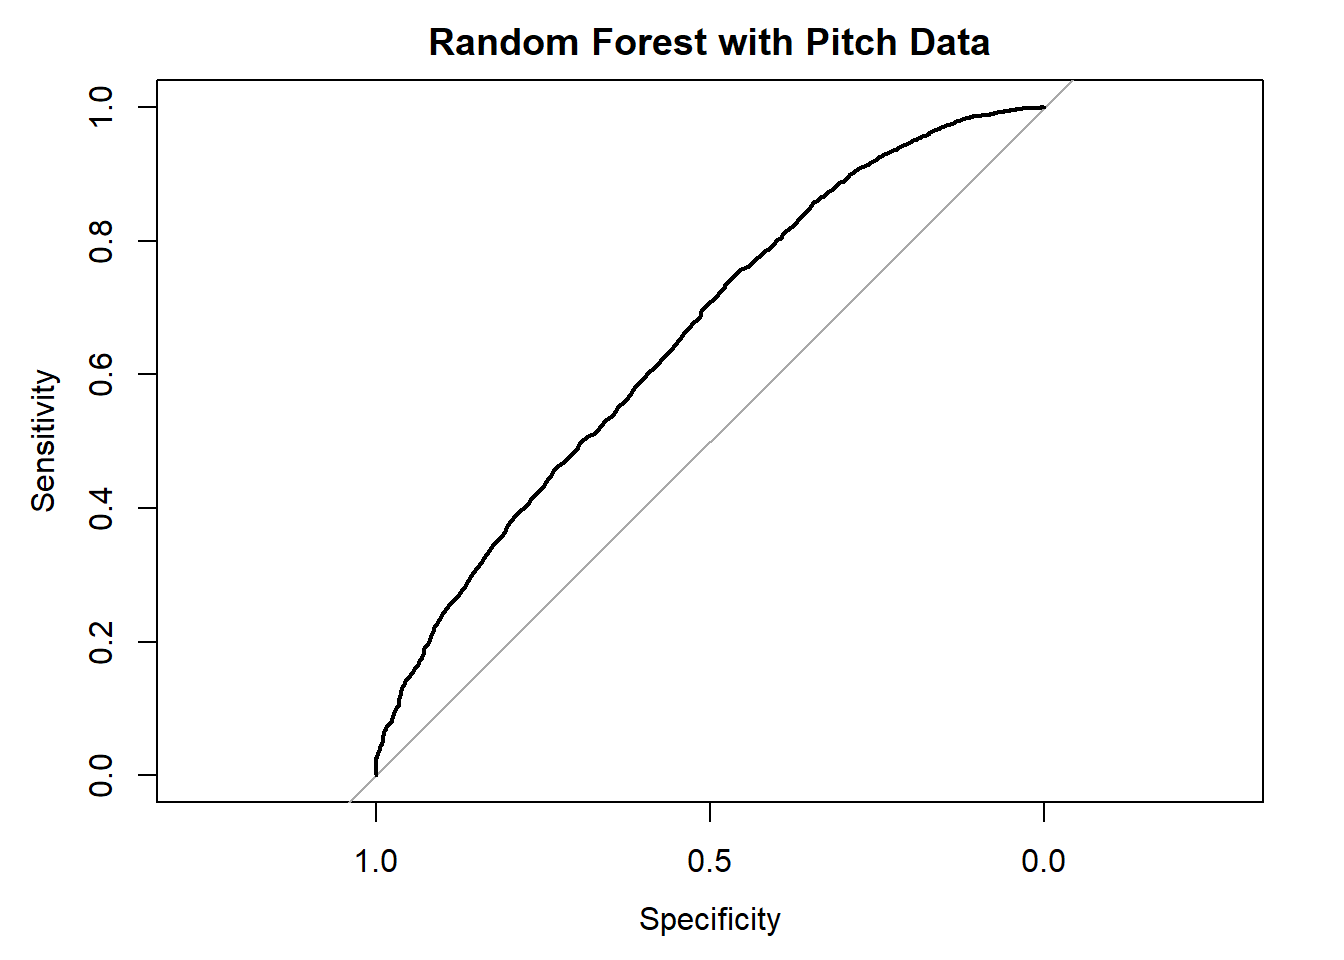
\includegraphics[height=2in]{images/full_rf_roc.png}
    \caption{ROC curves for the logistic regression model (left) and the random forest classifier (right) trained with pitch data included in the models.}
    \label{fig1_roc}
\end{figure}

\begin{figure}[h]
    \centering
    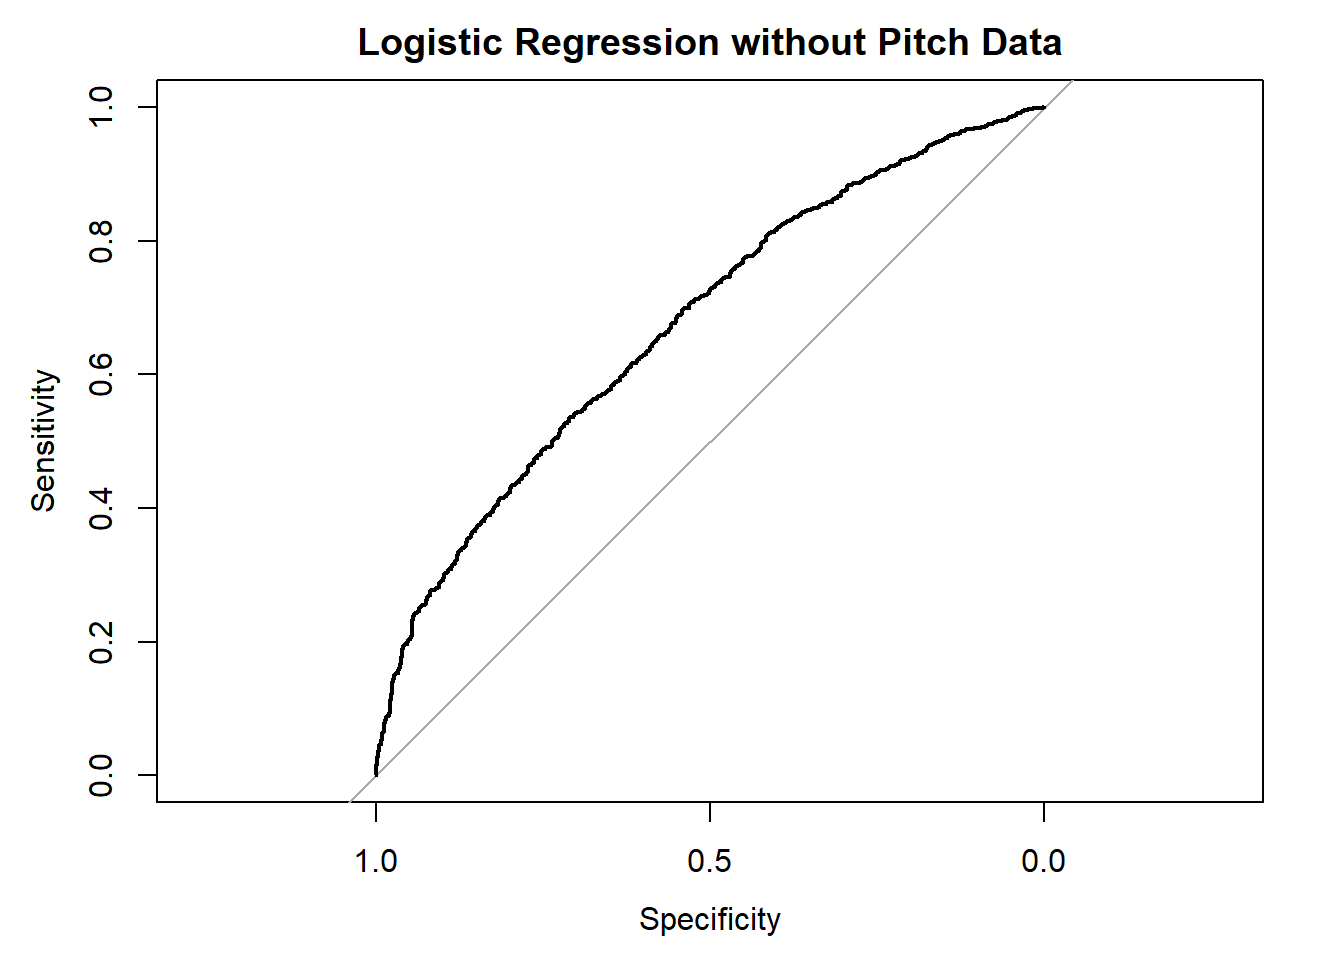
\includegraphics[height=2in]{images/reduced_pitchless_glm_roc.png}
    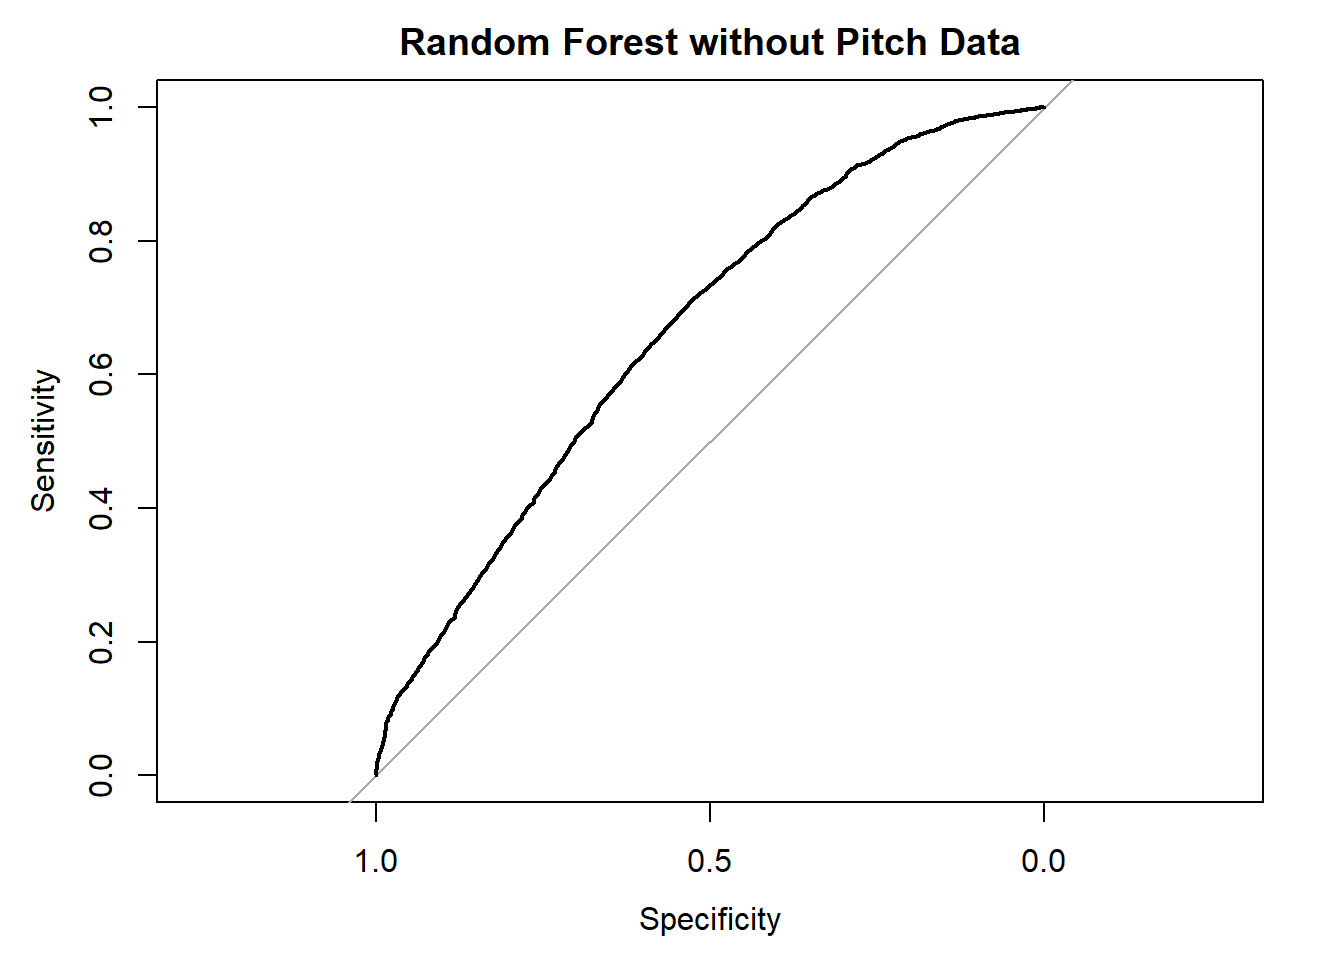
\includegraphics[height=2in]{images/pitchless_rf_roc.png}
    \caption{ROC curves for the logistic regression model (left) and the random forest classifier (right) trained with pitch data excluded from the models.}
    \label{fig2_roc}
\end{figure}

\newpage
\begin{figure}[h]
    \centering
    \subfloat[][]{
        \begin{tabular}{c c c c}
            \toprule
            && \multicolumn{2}{c}{Reference} \\
            && Failure & Success \\
            \multirow{2}*{Prediction}
                & Failure & 107 & 64 \\
                & Success & 573 & 1922 \\
            \bottomrule
        \end{tabular}
    }
    \qquad
    \subfloat[][]{
        \begin{tabular}{c c c c}
            \toprule
            && \multicolumn{2}{c}{Reference} \\
            && Failure & Success \\
            \multirow{2}*{Prediction}
                & Failure & 319 & 188 \\
                & Success & 1721 & 5770 \\
            \bottomrule
        \end{tabular}
    }
    \caption{Confusion matrices built using predictions from the logistic regression model (a) and the random forest (b) trained on the full data set (with pitch data).}
    \label{fig3_conf}
\end{figure}
\begin{figure}[h]
    \centering
    \subfloat[][]{
        \begin{tabular}{c c c c}
            \toprule
            && \multicolumn{2}{c}{Reference} \\
            && Failure & Success \\
            \multirow{2}*{Prediction}
                & Failure & 113 & 85 \\
                & Success & 705 & 1964 \\
            \bottomrule
        \end{tabular}  
    }
    \qquad
    \subfloat[][]{
        \begin{tabular}{c c c c}
            \toprule
            && \multicolumn{2}{c}{Reference} \\
            && Failure & Success \\
            \multirow{2}*{Prediction}
                & Failure & 553 & 369 \\
                & Success & 1901 & 5778 \\
            \bottomrule
        \end{tabular}
    }
    \caption{Confusion matrices built using predictions from the logistic regression model (a) and the random forest (b) trained on the reduced data set (without pitch data).}
    \label{fig4_conf}
\end{figure}

\begin{longtable}{c c c c c}
    \hline
    Coefficients & Estimate & Standard Error & z-value & Pr$(>|z|)$ \\
    \hline
    (Intercept) & -3.822 & 2.272 & -1.682 & 0.092 \\
    outs & 0.119 & 0.063 & 1.896 & 0.058 \\
    on\_third & 1.610 & 0.208 & 7.724 & $\approx 0$ \\
    num\_pitches & -0.192 & 0.029 & -6.729 & $\approx 0$ \\
    is\_hitters\_count & 1.171 & 0.300 & 3.908 & $\approx 0$ \\
    is\_pitchers\_count & 0.410 & 0.133 & 3.078 & 0.002 \\
    strike\_on\_event & -0.248 & 0.104 & -2.388 & 0.017 \\
    pitchout\_on\_event & -1.281 & 0.398 & -3.215 & 0.001 \\
    blocked\_on\_event & 1.321 & 0.326 & 4.053 & $\approx 0$ \\
    pitcher\_throws\_left & 0.250 & 0.126 & 1.988 & 0.047 \\
    batter\_bats\_left & -0.144 & 0.096 & -1.507 & 0.132 \\
    start\_speed & -0.039 & 0.009 & -4.383 & $\approx 0$ \\
    p\_fastball\_rate\_2018 & 0.600 & 0.424 & 1.414 & 0.157 \\
    r\_sb\_rate\_2017 & 0.446 & 0.265 & 1.687 & 0.092 \\
    r\_sprint\_speed\_2018 & 0.154 & 0.040 & 3.801 &  $\approx 0$ \\
    c\_pop\_2b\_sba\_2018 & 1.723 & 0.892 & 1.933 & 0.053 \\
    \hline
    \caption{Summary table for the logistic regression model trained on the full data set (including pitch data).}
    \label{tab3_logistic_summary}
\end{longtable}

\vspace{0.5cm}

\begin{longtable}{c c c c c}
    \hline
    Coefficients & Estimate & Standard Error & z-value & Pr$(>|z|)$ \\
    \hline
    (Intercept) & -8.171 & 1.984 & -4.119 & $\approx 0$ \\
    outs & 0.101 & 0.057 & 1.775 & 0.076 \\
    on\_third & 1.583 & 0.192 & 8.226 & $\approx 0$ \\
    num\_pitches & -0.207 & 0.028 & -7.286 & $\approx 0$ \\
    is\_hitters\_count & 0.895 & 0.255 & 3.516 & $\approx 0$ \\
    is\_pitchers\_count & 0.649 & 0.117 & 5.539 & $\approx 0$ \\
    pickoffs\_to\_first & -0.157 & 0.046 & -3.437 & 0.001 \\
    pitchouts & -0.703 & 0.347 & -2.026 & 0.043 \\
    pitches\_run\_on & 0.519 & 0.099 & 5.229 & $\approx 0$ \\
    r\_sb\_rate\_2017 & 0.455 & 0.247 & 1.844 & 0.065 \\
    r\_sprint\_speed\_2018 & 0.171 & 0.038 & 4.492 & $\approx 0$ \\
    c\_pop\_2b\_sba\_2018 & 1.779 & 0.800 & 2.223 & 0.026 \\
    \hline
    \caption{Summary table for the logistic regression model trained on the reduced data set (excluding pitch data).}
    \label{tab4_logistic_summary}
\end{longtable}

\vspace{0.25cm}

\begin{longtable}{c c c}
    \hline
    Variable & Mean Decrease in Accuracy & Mean Decrease in Gini Index \\
    \hline
    outs & 8.895 & 32.514 \\
    on\_third & 27.306 & 24.810 \\
    num\_pitches & 18.836 & 69.679 \\
    is\_hitters\_count & 4.006 & 5.490 \\
    is\_pitchers\_count & 4.343 & 14.153 \\
    strike\_on\_event & 5.895 & 16.447 \\
    swing\_on\_event & 3.830 & 13.610 \\
    pitchout\_on\_event & 7.639 & 4.483 \\
    blocked\_on\_event & 9.343 & 6.270 \\
    pickoffs\_to\_first & 5.217 & 37.944 \\
    pitchouts & 3.741 & 3.733 \\
    pitches\_run\_on & 7.750 & 12.903 \\
    b\_score\_difference & 1.013 & 60.411 \\
    pitcher\_throws\_left & 1.833 & 13.261 \\
    batter\_bats\_left & 1.833 & 18.646 \\
    start\_speed & 5.143 & 108.773 \\
    p\_sb\_rate\_2017 & 0.162 & 67.403 \\
    p\_pickoff\_rate\_2018 & 2.950 & 43.255 \\
    p\_fastball\_rate\_2018 & 1.738 & 102.696 \\
    r\_sb\_rate\_2017 & 6.064 & 87.110 \\
    r\_sprint\_speed\_2018 & 6.677 & 91.780 \\
    c\_sb\_rate\_2017 & 3.565 & 76.033 \\
    c\_pop\_2b\_sba\_2018 & 3.676 & 72.413 \\
    \hline
    \caption{Relative importance measures for the variables included in the random forest trained on the full data set (with pitch data). Higher scores indicate higher importance in the random forest.}
    \label{tab5_importance}
\end{longtable}

\vspace{0.25cm}

\begin{longtable}{c c c}
    \hline
    Variable & Mean Decrease in Accuracy & Mean Decrease in Gini Index \\
    \hline
    outs & 10.440 & 45.211 \\
    on\_third & 33.595 & 33.911 \\
    num\_pitches & 23.516 & 91.659 \\
    is\_hitters\_count & 2.214 & 6.313 \\
    is\_pitchers\_count & 4.706 & 22.332 \\
    pickoffs\_to\_first & 19.605 & 58.173 \\
    pitchouts & 7.742 & 7.016 \\
    pitches\_run\_on & 19.906 & 35.977 \\
    pitcher\_throws\_left & 3.422 & 20.094 \\
    batter\_bats\_left & -0.363 & 27.374 \\
    p\_sb\_rate\_2017 & 2.309 & 97.117 \\
    p\_pickoff\_rate\_2018 & 15.340 & 77.994 \\
    p\_fastball\_rate\_2018 & 3.446 & 149.983 \\
    r\_sb\_rate\_2017 & 6.678 & 126.495 \\
    r\_sprint\_speed\_2018 & 10.767 & 137.819 \\
    c\_sb\_rate\_2017 & 4.363 & 107.015 \\
    c\_pop\_2b\_sba\_2018 & 3.313 & 100.361 \\
    \hline
    \caption{Relative importance measures for the variables included in the random forest trained on the reduced data set (without pitch data). Higher scores indicate higher importance in the random forest.}
    \label{tab6_importance}
\end{longtable}


\subsection*{Appendix C: An Introduction to Logistic Regression}
\addcontentsline{toc}{subsection}{Appendix C: An Introduction to Logistic Regression}

Put simply, regression is a mathematical procedure for modeling the relationship between a response variable and some set of predictor variables. The most common form of regression is linear regression, which posits a linear relationship between the response variable (which is usually continuous) and the predictor variables. The model equation is \[Y = \beta_0 + \beta_1x_1 + \beta_2x_2 + \dots + \beta_kx_k,\] where $Y$ is the response variable, the $x_i$'s are the predictor variables, and the $\beta_i$'s are the unknown model parameters. The goal of linear regression is to estimate these unknown parameters, using a set of training data, so that the resulting model produces estimated values of the response variable that most closely match the observed values of the response variable in the data set. The least-squares method is the most common strategy for finding these estimates.

While linear regression performs well for continuous response variables, it is not appropriate to use on a categorical response variable. In particular, a binary response variable (such as the outcome of a stolen base attempt) requires a modified approach to regression, called logistic regression. The goal of logistic regression is to use a set of predictor variables to explain the odds that a binary outcome will be a ``success,'' as opposed to a ``failure.'' So, instead of assuming a linear relationship between the predictor variables and the response variable itself, a logistic regression model posits a linear relationship between the predictor variables and the log odds of success for the response variable \citep{peng}. The model equation is \[\log \frac{p}{1-p} = \beta_0 + \beta_1x_1 + \beta_2x_2 + \dots + \beta_kx_k,\] where $p$ is the probability of success. Transforming the log odds of success into simply the probability of success, the model equation can also be written as \[p = \frac{e^{\beta_0 + \beta_1x_1 + \beta_2x_2 + \dots + \beta_kx_k}}{1 + e^{\beta_0 + \beta_1x_1 + \beta_2x_2 + \dots + \beta_kx_k}}.\]

With this model equation and a training data set, maximum likelihood estimation is usually employed to fit the model. Maximum likelihood estimation works by finding the estimates of the model parameters that, taken together, maximize the likelihood of the observed data appearing as they do. After the parameters are estimated, estimating the probability of a successful binary outcome is as simple as plugging in values for each predictor variable into the above model equation.

As with any parametric model, the logistic regression model makes important assumptions about the variables and the data used in fitting the model. Most notably, it is assumed that each observation in the data set follows a Bernoulli probability distribution and that the observations are independent of each other. In the case of this thesis, the logistic regression model assumes that different stolen base attempts are independent of each other, implying that the probability of success of any given stolen base attempt has no impact on or correlation with the probability of success of any other stolen base attempt. This assumption may not be completely valid, as different stolen base attempts that involve the same pitcher, baserunner, or catcher may be correlated. Different stolen base attempts from one very fast baserunner, for example, are likely to all have a relatively high probability of success. One possible strategy to address the presence of correlated observations involving the same players is to employ a mixed-effects model, which accounts for the effect of having the same individual appear in several different observations. However, there is such a large number of different pitchers, baserunners, and catchers in this data set that a mixed-effects model would be quite complex and unwieldy. Furthermore, the primary goal of this project is to produce the best possible model in terms of predictive ability -- whether the model is a perfect fit for the data is of secondary concern.



\subsection*{Appendix D: An Introduction to Random Forests}
\addcontentsline{toc}{subsection}{Appendix D: An Introduction to Random Forests}

A random forest is an ensemble method for classification, built as an aggregation of a large number of decision tree classifiers \citep{hitchcock}. A decision tree classifier fulfills the same goal as a logistic regression model -- classifying the outcome of a categorical (or in particular, binary) response variable according to some number of predictor variables. However, unlike a logistic regression model, a decision tree is nonparametric, meaning it places no prior assumptions on the distribution of the data. As a result, there are no model parameters to estimate in a decision tree. Instead, the tree is built by repeatedly partitioning the training data set according to the values of the predictor variables, with the hope that the data set can be perfectly separated into groups corresponding to each category of the response. Every branch of the tree represents a splitting rule for the data based on a particular predictor variable, and the two child nodes of a branch represent the two subsets of the data created by the splitting rule. Ideally, every leaf node in the tree will only contain observations that share the same category of the response variable (for the stolen base data, every leaf node should either contain all successes or all failures). In most cases, though, it is impossible for a decision tree to produce completely ``pure'' leaf nodes. Instead, the goal is to maximize the node purity. For every possible predictor variable, a splitting rule based on that predictor is designed so that each of the two subsets created by the splitting rule is as uniform as possible in terms of the category of the response variable. 

To classify the response of a new observation using a decision tree, it is possible to use the values of the observation's predictor variables to follow the branches of the tree (the splitting rules) until a leaf node is reached. The category that is most prevalent in this leaf node is the category predicted for the new observation. For a more complex approach to classification, random forests are used. In a random forest, a large number of decision trees are created, using different subsets of the predictor variables and different splitting rules. Then, a new observation is classified by performing classification in each of the decision trees and choosing the category of the response which most commonly appears as a prediction across all of the trees. It is also possible to obtain an estimated probability for the classification of each category by calculating the proportion of the decision trees which predict that category. For example, the estimated probability of success for a stolen base attempt produced by a random forest is simply the proportion of the decision trees which classify the attempt as successful.  



\end{document}